\chapter{Why Computer Networks Matter}

Consider this: when you send a short message from your phone, it may travel thousands of kilometers across the globe—passing through a network of undersea cables, satellites, and data centers—before it appears on someone else’s screen. This entire journey takes place in less time than the blink of an eye. Behind this seamless experience lies a highly sophisticated system known as computer networking. Though often invisible to the average user, it is this system that enables everything from global communication to real-time collaboration and digital commerce. In this chapter, we will explore why computer networks matter, how they have shaped the modern world, and why understanding them is essential in the digital age.

\begin{figure}[H]
    \centering
    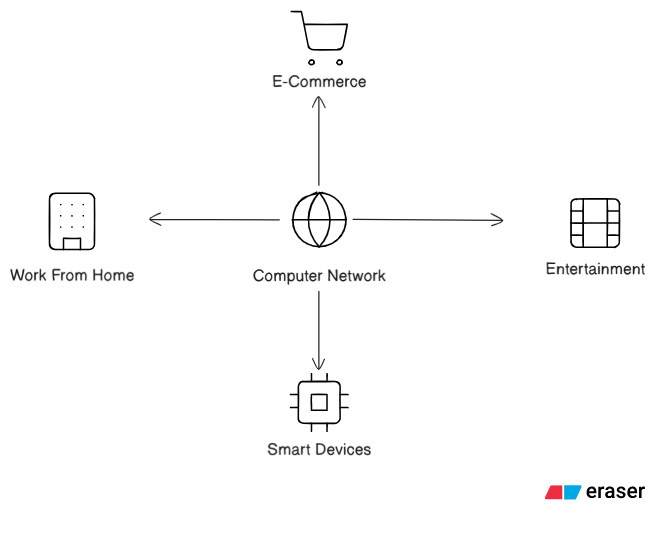
\includegraphics[width=0.4\textwidth]{images/chapter1/fig1.png}
    \caption{Computer Network Connecting The World}
    \label{fig:why-cn-matters}
\end{figure}

\section{What is a Computer Network?}

\begin{figure}[H]
    \centering
    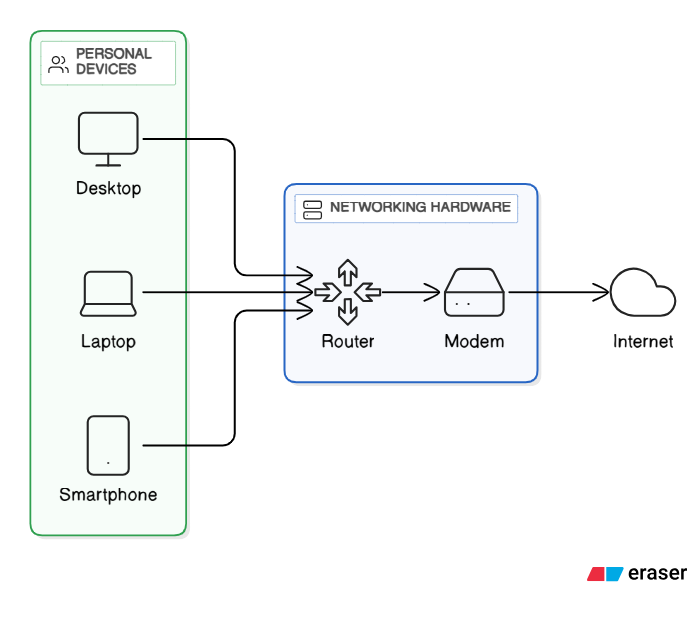
\includegraphics[width=0.6\textwidth]{images/chapter1/fig2.png}
    \caption{Basic Computer Network}
    \label{fig:basic-cn}
\end{figure}

A computer network is a system of interconnected devices—such as computers, servers, mobile phones, and other hardware—that communicate and share data with each other using a set of rules known as network protocols.

In simpler terms, it is a collection of devices linked together to exchange information, share resources (like files, printers, or internet access), and enable communication over short or long distances.

At the core of every network is the principle of data transmission—the ability to send digital information (such as text, audio, video, and files) from one point to another, often in real time.

\begin{examplebox}
    For instance, when a student accesses an online lecture from their laptop, they are using a computer network. Their request travels through Wi-Fi, reaches a local router, moves through a series of internet service providers (ISPs), and eventually connects to a remote server hosting the video—all within seconds.
\end{examplebox}

\section{Evolution of Computer Networks}

The evolution of computer networks began in the 1960s with the concept of packet switching, introduced by researchers like Paul Baran and Donald Davies. This method of data transmission laid the foundation for modern networking. In the 1970s, the U.S. Department of Defense developed ARPANET, the first operational packet-switched network, connecting universities and research centers. The 1980s marked a major breakthrough with the introduction of the TCP/IP protocol, which allowed different networks to communicate reliably and led to the formation of the internet. In the 1990s, Tim Berners-Lee invented the World Wide Web, turning the internet into a global system of interlinked documents and websites, making it accessible to the general public. The 2000s saw the rise of the commercial internet, with the emergence of e-commerce, social media, and broadband connectivity, making the internet a central part of everyday life.

\begin{figure}[H]
    \centering
    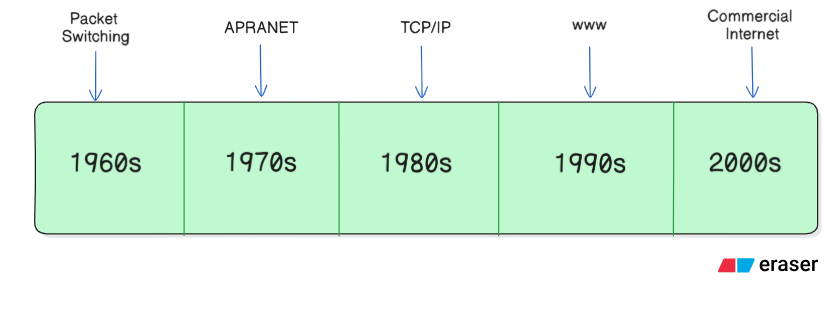
\includegraphics[width=0.8\textwidth]{images/chapter1/fig3.png}
    \caption{Evolution of Computer Networks}
    \label{fig:evolution-of-cn}
\end{figure}



\begin{didyouknowbox}
    Did you know that the first message ever sent over the ARPANET (the precursor to the internet) was "LO"? The intention was to send "LOGIN," but the system crashed after just two letters!
\end{didyouknowbox}


\section{Real World Relavance of Computer Networks}
Computer networks are not just technical constructs; they have real-world implications that affect nearly every aspect of our lives. From enabling remote work and online education to facilitating e-commerce and social media, networks have transformed how we interact, learn, and conduct business.
In healthcare, networks allow for telemedicine, enabling doctors to consult with patients remotely. In education, they support online learning platforms that provide access to resources and courses from anywhere in the world. In business, networks enable global collaboration, allowing teams to work together seamlessly regardless of their physical locations.
\begin{casestudybox}
    Consider the case of a multinational corporation with offices in different countries. Their employees rely on computer networks to share documents, hold video conferences, and access centralized databases. This connectivity not only enhances productivity but also fosters innovation by allowing diverse teams to collaborate effectively.
\end{casestudybox}

\section{How Networks Changed the World}
The development of computer networks has been one of the most transformative technological shifts in human history. By enabling seamless data exchange and global communication, networks have fundamentally reshaped the way we live, work, and connect.

\begin{description}
    \item \textbf{Global Communication:} Emails, Instant messaging, and social media platforms allow people to communicate across vast distances in real time, breaking down georgraphic barriers and fostering global connections.
    \item \textbf{Information Access:} The internet, a vast network of networks, provides access to an unprecedented amount of information. Search engines, online libraries, and educational platforms have democratized knowledge, making it available to anyone with an internet connection.
    \item \textbf{E-commerce:} Online shopping has revolutionized retail, allowing consumers to purchase goods and services from anywhere in the world. This has led to the rise of global marketplaces and has transformed traditional business models.
    \item \textbf{Remote Work:} The COVID-19 pandemic accelerated the adoption of remote work, highlighting the importance of computer networks in enabling employees to work from home. Video conferencing tools, cloud services, and collaborative software have become essential for maintaining productivity and communication in a distributed work environment.
\end{description}

\section{Conclusion}

Computer networks have become the invisible infrastructure powering the digital age. From the moment we send a message or access a website, to complex operations like remote surgeries or global stock exchanges, networks make it all possible. As we've seen, they are not just technical systems—they are enablers of communication, education, commerce, healthcare, and innovation.

Understanding computer networks is essential not only for those pursuing careers in technology but also for anyone living in a digitally connected world. As networks continue to evolve—with advancements like 5G, edge computing, and the Internet of Things (IoT)—their role in society will only become more critical.

In the chapters ahead, we will dive deeper into the types of networks, how they are structured, the devices that make them work, and the protocols that allow them to function efficiently and securely.
